\section{Empirical evidence for nonnegative sparse coding in the brain}

\subsection{Reconstructing stimulus spaces using sparse, parts-based representations}

An influential paper by Lee and Seung \citep{LeeSeung1999},
found that applying a linear dimensionality reduction technique
known as \ac{NMF} to a database of face images
yielded sparse, localized features that resembled parts of a face \citep{Wachsmuth1994},
which is a an area in the ventral visual ``what'' stream
that responds to objects as a whole
\citep{ungerleider1994and}.
\ac{NMF} is a statistical matrix decomposition technique 
that takes an $F \times S$ data matrix \textbf{V} 
whose rows correspond to distinct features of the input 
(e.g., $F$ different pixels of an image)
and whose columns correspond to different stimuli or 
observations of those features
(e.g., $S$ different images). 
Matrix \textbf{V} must be nonnegative, and \ac{NMF} decomposes the matrix into two reduced-rank matrices whose linear combination can be weighted such that the product of \textbf{W} and \textbf{H} provides an accurate reconstruction of \textbf{V} (Fig.~\ref{fig:NMF|reconstruction}).
\jeffNote{The above paragraph does not agree with my understanding of area IT.  I thought IT responded to whole objects not parts. Also, Lee and Seung never mention IT in their paper. In fact, they never mention cortex! Be precise with your claims.}

On its surface, NMF would appear to be unrelated to the mechanisms underlying 
artificial or biological neural networks;
however, it was Lee and Seung's intuitive mapping of these variables onto
a neural network that forms the cornerstone of our conception of the NSC framework:
A particular image, in this case encoded by $F = 19 \times 19 = 361$ 
pixels $v_1, \ldots, v_F$
(i.e., a column of \textbf{V}),
could be reconstructed by a linear mixing of a total of $B$ encoding variables
$h_1, \ldots, h_B$ (i.e., a column of \textbf{H}).
A single encoding variable $b \in 1, \ldots, B$ 
influences multiple image pixels,
owing to the fan-out of the connections from the encoding variable.
As a result, a particular image of a face (Fig.~\ref{fig:NMF|reconstruction}B1)
could be accurately represented by a linear combination of 
only $B = 49$ encoding variables or ``basis images''.
Similar to the preferred stimuli of
neurons in inferotemporal cortex \citep{Wachsmuth1994},
these basis images resembled parts of faces,
which could be additively combined to represent a whole face.
\jeffNote{Can you make sure what was found in 1994 still agrees with what we now know goes on in area IT?}

% In this experiment, the network was trained on a database of  2,429 facial images, but the dimensionality of the resulting basis matrix \textbf{W} was 49.\emilyNote{added dimensionality reduction}
% \jeffNote{somewhere around here you should say how much the dimensionality is reduced (size of W and H) for each example in figure 1}
Remarkably, such a parts-based representation is not specific to
% \mikeNote{I moved the bit about the what pathway up to where we first mention IT}
information processing in inferotemporal cortex; 
the same principle can be extended to other areas of the visual system,
such as the \ac{MSTd},
which is part of the visual motion pathway \citep{Beyeler2016}.
Neurons in \ac{MSTd} respond to relatively large and complex patterns
of retinal motion (``optic flow''),
owing to input from direction and speed selective neurons in the \ac{MT}
(for a recent review, see \cite{Orban2007}).
Although \ac{MSTd} had long been suspected to be involved in the
analysis of self-motion,
the complexity of neuronal response properties has made it difficult
to experimentally investigate how neurons in \ac{MSTd}
might perform this function.
However, when Beyeler and colleagues \citep{Beyeler2016}
applied \ac{NMF} to \ac{MT}-like patterns of activity,
they found a sparse, parts-based representation of retinal flow
(Fig.~\ref{fig:NMF|reconstruction}B2)
similar to the parts-based representation of faces
encountered by Lee and Seung \cite{LeeSeung1999}.
The resulting ``basis flow fields'' showed a remarkable resemblance to receptive fields
of \ac{MSTd} neurons, as they preferred an intricate mixture of
3D translational and rotational flow components
in a subset of the visual field.
% \mikeNote{What about this? Avoiding ``dimensionality of a matrix'' again, and highlighting the usefulness of such a representation}
As a result, any flow field possibly to be encountered 
during self-movement through a 3D environment
could be represented by a linear combination
of only $64$ basis flow fields.
\jeffNote{64 means nothing to me unless you can say what it was reduced from. Also, you need to report the sparsity in the MSTd experiments.}
% The dimensionality of the basis matrix \textbf{W} in this experiment was also dramatically reduced. The model was trained on a set of 6,000 flow fields, which was reduced to only 64 basis flow fields after the application of NMF.\emilyNote{added dimensionality reduction}
\mikeNote{Figure 1: Kris is right, A should show the third column of H, same as W... Emily, do you still have the raw version of A?}
\emilyNote{I have the powerpoint but I can't edit the schematic of A. I tried to ungroup it but it looks like whenever you sent to me it saved the panel as a whole image.}

\jeffNote{fix caption in key figure}


\begin{figure}[h]
	\centering
	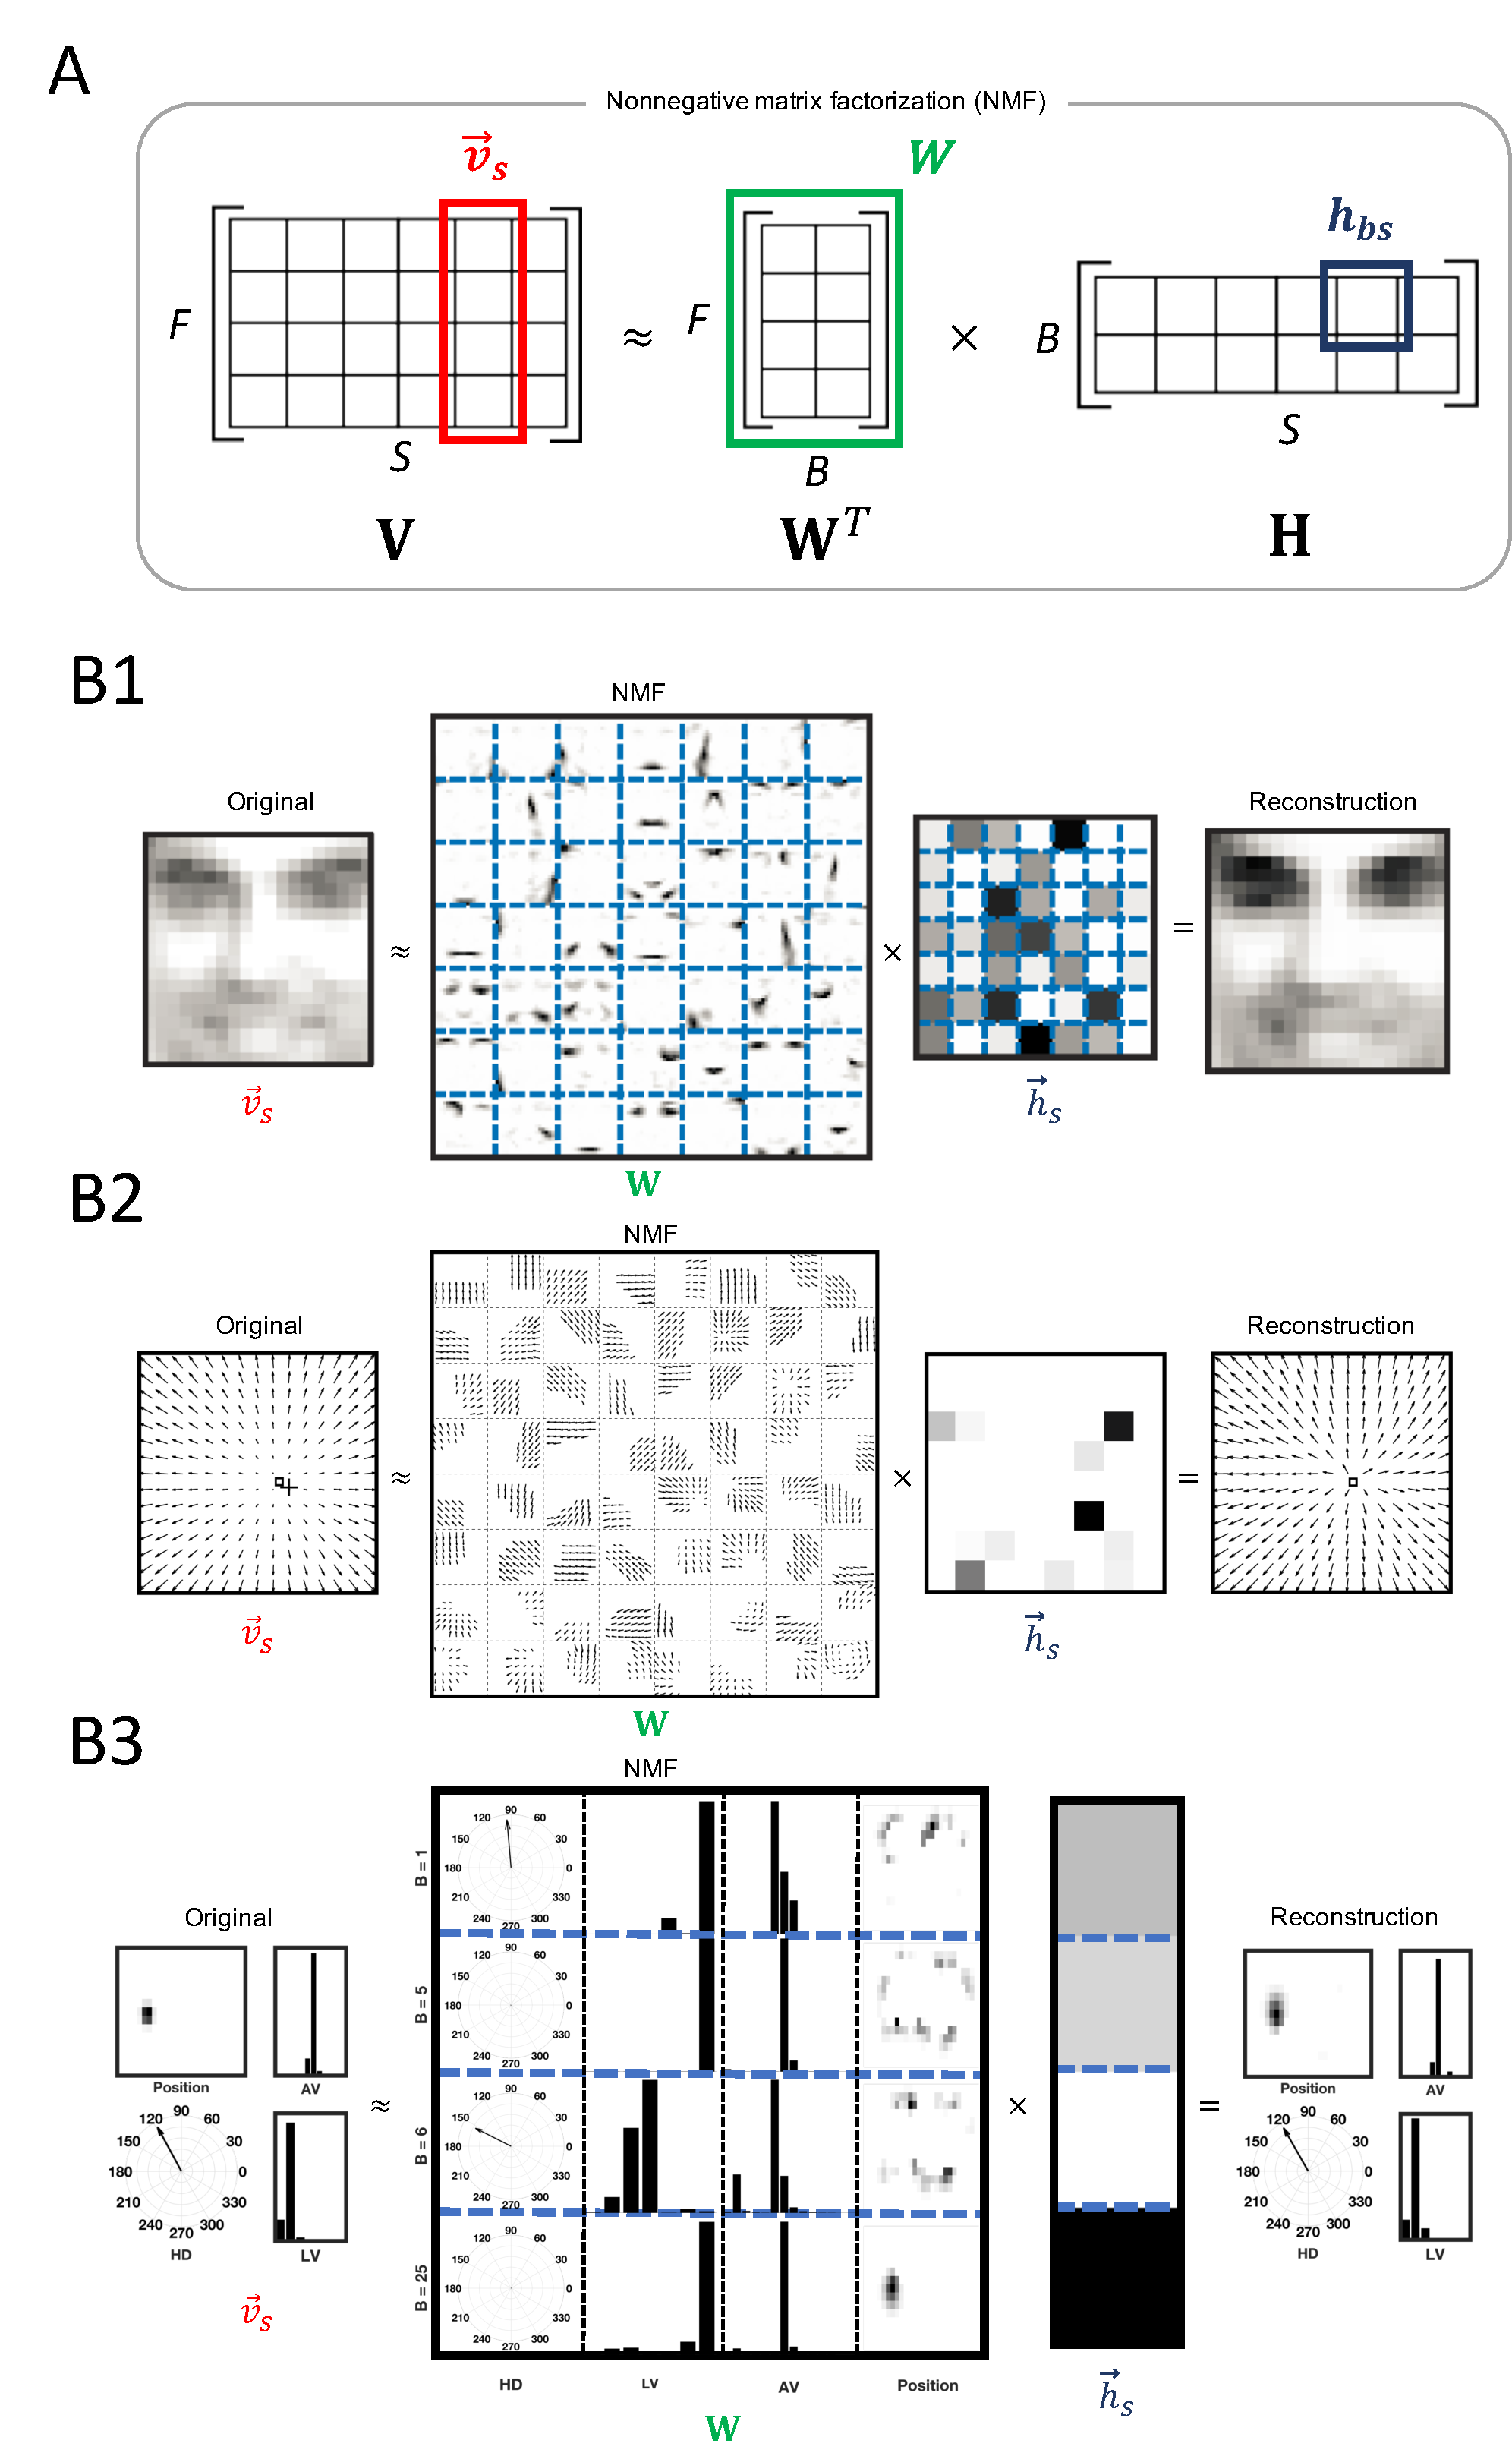
\includegraphics[scale=0.17]{keyFig_fixed}
    \caption{(Key Figure) \ac{NMF} can recover sparse, parts-based
         representations of high-dimensional input data.
         A)  A data matrix \textbf{V} ($F$ features x $S$ stimulus
             observations) can be reconstructed from two reduced-rank
             matrices \textbf{W} (containing $B$ basis vectors) and 
             \textbf{H} (containing the hidden coefficients of the
             decomposition).
             Any individual input stimulus (i.e., column in \textbf{V})
             can be reconstructed from a linear combination of a set of
             basis vectors (i.e., the columns in \textbf{W}).
         B1--B3) Recovered weight matrices \textbf{W} resemble the
             receptive fields of cortical neurons across brain regions. The contribution of each basis vectors is given by a column 
             in \textbf{H} (the darker the color, the stronger the
             contribution).
             % I know I'm conflating synaptic weights and RFs here, but
             % I don't know how to say it better without being too wordy.
         B1) A facial image can be reconstructed from a sparse activation
             of simulated neurons in inferotemporal cortex that
             preferentially respond to parts of faces
             (adapted from \cite{LeeSeung1999}).
         B2) An optic flow field can be reconstructed from a sparse
             activation of \ac{MSTd} neurons that prefer various
             directions of 3D self-translation and self-rotation
             (adapted from \cite{Beyeler2016}).
         B3) A rat's allocentric position and route-based direction of
             motion can be reconstructed from a sparse activation of
             model \ac{RSC} neurons that prefer an intricate combination of
             linear velocity (LV), angular velocity (AV), head direction (HD)
             and position (Position). Only the ??? 4 most contributing hidden coefficients out of ??? are shown for the
             sake of clarity.}
	\label{fig:NMF|reconstruction}
\end{figure}

% Schematic of matrix decomposition under NMF with representative examples. (A) An input vector or matrix V can be decomposed into components W and H, in which W corresponds to the parts-based basis functions that can be added up linearly to reconstruct the original input. W is a vector whose length is equal to the number of elements needed to reconstruct the input space. H represents the hidden coefficients used to weight the basis functions in H accordingly in order to reconstruct the input space.  In an artificial neural network, V again represents the inputs to the network, H corresponds to the hidden neurons that represent the features that correspond to the input to the network, and W represents the synaptic weights between the input neurons encoding the input V and the hidden neurons H. (B) Top, adapted from Lee \& Seung, 1999, shows the resulting decomposition of NMF when applied to images of faces. The weight matrix W is intuitively parts-based and seems to correspond to individual facial features. When multiplied by a particular column of H associated with a particular face, that face can be reconstructed. Middle, NMF was applied to MT-like input patterns and successfully produced a parts-based representation of retinal flow. Bottom, NMF was applied to idealized neural representations of certain behavioral features and produced a parts-based representation of space anchored to multiple spatial frames of reference, similar to neuronal responses in the biological brain area RSC.
% Caption is at 240 words currently

% Overall, the sparse decomposition model \cite{Beyeler2016} provides 
% strong theoretical evidence
% that \ac{MSTd} neurons might decompose optic flow,
% in the sense of matrix factorization,
% to reduce the number of ``templates'' used to represent the spectrum of
% retinal flow fields encountered during self-movement
% in an efficient and parsimonious fashion.
% Thus commonly observed response properties,
% such as complex motion tuning and heading selectivity,
% might simply be a by-product of \ac{MSTd} neurons performing a biological equivalent
% of dimensionality reduction on their inputs.


Analogously, NSC can explain response properties
of neurons outside the visual system, 
such as in the \ac{RSC}, an area important for navigation and spatial memory \cite{Miller2014,Nelson2015,VannAggleton2009}.
Neurons in the \ac{RSC} conjunctively encode multiple variables related to 
the environment and one's position and movement within it,
allowing the representation of spatial features of the environment 
with respect to multiple reference frames \cite{AlexanderNitz2015}.
However, establishing a mechanistic link 
between physiological response properties of \ac{RSC} neurons 
and their underlying representations of space
has proved difficult,
due to the complexity of their response properties and because inputs to the region are not easily isolated.
Yet by applying \ac{NMF} to idealized input neurons that encoded 
experimentally recorded behavioral variables 
associated with rats running along a track, we were able to replicate
functionality observed in the biological \ac{RSC} (Fig.~\ref{fig:NMF|reconstruction}B3). Once again, the dimensionality was massively reduced from a set of 1,017 input neurons to a set of 30 basis functions.
% \mikeNote{Too soon?}
% The same results were obtained when evolutionary algorithms 
% were used to optimize the metaparameters associated with \ac{STDPH}
% on a population of \acp{SNN} that replicated 
% the same dataset \citep{Rounds2016}.

Although there seems to be a consensus that information-theoretic explanations are relevant when investigating the early visual system,
higher-order brain areas are often considered to be specialized for
performing tasks
(e.g., recognizing objects, making decisions, navigating an environment),
rather than efficiently encoding of information.
However, the finding that \ac{NSC} could be used to explain
neuronal responses in the visual and retrosplenial cortices
introduces the possibility that it might apply elsewhere in the brain.
In fact, sparse
(and potentially parts-based)
representations have been in 
olfactory, auditory, somatosensory, 
and motor cortices
(Table \ref{table:listEvidence}). 
This introduces the possibility that \ac{NSC} might in fact
be a general principle to which neuronal computations adhere.

\begin{table}[ht]
	\centering
    % Mike: Shortened description
	\caption{Nonnegative sparse coding in the brain.
    We list a group of brain regions for which there is experimental evidence of certain features associated with NSC (`X': evidence exists, `?': has yet to be investigated).
   For each brain region, the left-hand side of the table lists experimental evidence for sparse and/or parts-based representations, whereas the right-hand side lists computational support that NSC can describe receptive fields or response properties within that region.}
%     The table is divided into two parts for experimental and computational evidence. On the left columns, cells contain an `X' if a feature has been observed experimentally (sparse coding and/or parts-based representation), and a `?' is placed if there is no evidence for that feature in that region yet. The next column cites the studies where such features have been reported. On the right side of the table, we list whether NSC or NMF can describe receptive fields or response properties in the brain region with another `X,' or a `?' if no evidence exists. Again, beside this column, we cite the studies which have successfully modeled some aspect of the region using an NSC-like method.}    
    \scriptsize
	\begin{tabular}{r|rrr|rr}
	 &  &  \textbf{Parts-} & \textbf{Experimental} & \textbf{Modeled} & \textbf{Computational} \\
	\textbf{Area} & \textbf{Sparse} & 		\textbf{based} & \textbf{evidence} & \textbf{by NSC} & \textbf{ support} \\ \hline
    Retina & X & X & \cite{Onken2016} & X & \cite{Onken2016} \\
    Early visual cortex & X & X & \cite{OlshausenField1996,HoyerHyvarinen2002,Hoyer2003,vanHateren1998} & X & \cite{OlshausenField1996,Hoyer2003,Carlson2013,Hyvarinen2001} \\
    Ventral visual stream & X & X & \cite{Wachsmuth1994} & X & \cite{LeeSeung1999,Hosoda2009}  \\
    Dorsal visual stream & X & X & \cite{BenHamed2003,PougetSejnowski1997,PougetSnyder2000} & X & \cite{Beyeler2016} \\
    Auditory cortex & X & ? & \cite{Hromadka2008} & ? & ? \\
    Olfactory cortex & X & ? & \cite{Koulakov2011} & ? & \cite{MorenoBoteDrugowitsch2015}  \\
    Retrosplenial cortex & X & X & \cite{AlexanderNitz2015} & X & present paper \\
    Motor cortex & X & ? & \cite{GrazianoAflalo2007,Turner2000} & ? & \citep{Vargas2010decoding} \\
    Basal ganglia & X & ? & \cite{BarGad2000, BarGad2003_Review}  & X & \cite{BarGad2003_Review}, advanced RDDR \\
    Barrel cortex & X  & ? & \cite{Kerr2007} & ? & ?  \\
    Hippocampus & X & ? & \cite{Poli2017} & ? & ? \\
	\end{tabular}
    \label{table:listEvidence}
\end{table}


% The sparsity and nonnegativity constraints of the \ac{NSC} seem to extract similarities between neuronal firing patterns that result in
% consistent and stable representations, 
% while other statistical methods of dimensionality reduction 
% instead extract differences in firing patterns, thus capturing underlying representations of the data that are less stable and consistent, and are often less sparse. However, the exact implementation of dimensionality reduction in any given part of the brain might vary with the structure, and connectivity of the region.

